%
% teil2.tex -- Beispiel-File für teil2 
%
% (c) 2020 Prof Dr Andreas Müller, Hochschule Rapperswil
%
% !TEX root = ../../buch.tex
% !TEX encoding = UTF-8
%
\section{Parallelisierung
	\label{parallelisierung:sec:Parallelisierung}}
\kopfrechts{Parallelisierung}
Wir kennen nun numerische Verfahren, welche es einer Maschine erlaubt, unsere Feldgleichungen zu lösen.
Wir wissen auch, wie wir unser Feld in Teilgebiete unterteilen können.
Das gibt uns alle Werkzeuge, welche wir benötigen um die Berechnungen unserer Gleichungen auf mehrere Maschinen aufzuteilen.

Bei der Parallelisierung von Feldgleichungen in einem Multiprozessorsystem wird jedem Prozessor eines oder mehrere zusammenhängende Teilgebiete zugewiesen.
\index{Multiprozessorsystem}%
Die Teilgebiete müssen theoretisch nicht zusammenhängend sein, aber um die Kommunikation zwischen Prozessoren zu minimieren, ist dieses Vorgehen sinnvoll und üblich.
Da die Randzellen jedes Teilgebietes abhängig von den angrenzenden Zellen sind, siehe Abschnitt \ref{parallelisierung:sec:Gebietsunterteilung}, müssen die vorhandenen Informationen dieser Zellen zwischen Gebieten auf unterschiedlichen Prozessoren ausgetauscht werden.
Dieser Austausch ist mit erheblichem zeitlichen Aufwand verbunden.
Die Frage, wie fein ein Gitter in verschiedene Teilgebiete aufgeteilt werden soll, ist also immer eine Optimierungs-Frage.
Man muss ein Optimum finden, wo der zeitliche Gewinn der parallelen Berechnung die zeitlichen Verluste der Interprozess-Kommunikation überwiegt.

%
% einleitung.tex -- Beispiel-File für die Einleitung
%
% (c) 2020 Prof Dr Andreas Müller, Hochschule Rapperswil
%
% !TEX root = ../../buch.tex
% !TEX encoding = UTF-8
%
\subsection{Kommunikation zwischen Gebieten
\label{parallelisierung:sub:Interprozess}}
Zuerst eine kurze Rekapitulation zu einigen Begrifflichkeiten, welche wichtig sind für die Welt der parallelen Programmierung.
Ein Prozessor ist eine physische Recheneinheit wie zum Beispiel eine CPU oder GPU.
Prozessoren sind meist aus mehreren Kernen aufgebaut.
Jeder Kern ist eine eigenständige Recheneinheit und hat privaten wie auch mit anderen Kernen geteilten Speicher.
Ein Prozess ist ein eigenständiges Programm, welches vom Betriebssystem alle nötigen Resourcen wie Speicher, Rechenzeit und Daten zugeteilt bekommt.
Threads sind Teilaufgaben eines Prozesses, die gleichzeitig auf den verschiedenen Kernen des Prozessors arbeiten und sich die Daten und den Speicher dieses Prozesses teilen.

Für das Austauschen von Daten zwischen Teilgebieten gibt es zwei häufig verwendete Parallele Programmier- und Kommunikationsschnittstellen, OpenMP und MPI.
Im folgen werden beide kurz vorgestellt.

\subsubsection{OpenMP}
OpenMP ist eine API, welche sehr einfach das erzeugen von Threads und die Kommunikation zwischen diesen ermöglicht.
Jedes Teilgebiet wird hier einem Thread zugeteilt. 
Da sich diese Threads den Speicher des Prozesses teilen, nutzt OpenMP Shared-Memory für den Austausch von Daten.
Bei OpenMP gibt es keinen Thread-eigenen Speicher.
Jeder Thread kann also auf die Randzellen anderer Threads zugreifen.
Dadurch benötigt es keine Kommunikation zwischen den Teilgebieten im engeren Sinn.

Für kleine Systeme ist OpenMP eine einfache und gute Lösung.
Da es aber auf Shared-Memory basiert ist es schlecht skalierbar.
Werden für grosse Berechnungen mehrere Prozessoren verwendet ist Shared-Memory oft nicht verfügbar.
Grosse Berechnungen möchte man oft auch auf verschiedene Maschinen aufteilen, was mit OpenMP nicht möglich ist.
Der einfache Aufbau für den Programmierer bedeutet außerdem weniger Kontrolle über die Datenverteilung.

\subsubsection{MPI}
MPI ist ein Message Passing Interface.
Es dient nicht dazu Prozesse oder threads zu erzeugen.
Diese Aufgabe muss vom Betriebssystem ausgeführt werden.

MPI stellt Funktionen zur Verfügung für eine effiziente Kommunikation mittels Nachrichten zwischen den Prozessen.
Diese Prozesse haben nicht zwingend einen Shared Memory bereich.
Es wird daher als Distributed-Memory-Programmiermodell bezeichnet.
Jedes Teilgebiet wird hier einem Prozess zugeteilt.
Die Informationen über angrenzende Teilgebiete wird mittels Nachrichten oder auch Messages zwischen den Prozessen ausgetauscht.
Der Programmierer muss explizit Datenverteilung und Kommunikation steuern, was zwar einiges mehr Programmieraufwand aber auch bessere Kontrolle über die Daten bedeutet.

MPI zeichnet sich besonders über eine gute Skalierbarkeit aus.
Da kein Shared Memory nötig ist, kann man über beliebig viele Knoten, zum Beispiel mehrere CPUs oder ganze Rechner, die Daten durch Messages austauschen.

Man kann MPI auch für Systeme mit Shared Memory als eine Art Universallösung verwenden.
In diesem Fall wird allerdings trotz einem geteiltem Speicherbereich erheblicher Overhead für Kommunikation produziert, welcher mit OpenMP vermieden werden könnte.


\subsection{Beispiel an der allgemeinen Wärmeleitungsgleichung
	\label{parallelisierung:sub:BeispielParallelisierung}}
Zum besseren Verständnis wollen wir mit OpenMP ein konkretes Beispiel für die Parallelisierung der allgemeinen Wärmeleitungsgleichung realisieren.
Zum Vergleich wird auch die serielle Vorgehensweise präsentiert.
Als Ausgangslage soll für ein Gitter von $A \cdot B$ Zellen $C$ Updates durchgeführt werden.
Für jedes Update wird die Formel \eqref{parallelisierung:eq:update_formel} aus Abschnitt \ref{parallelisierung:sec:update_formel} verwendet.
Links und rechts der Zellen gibt es Reihen mit unveränderlicher Temperatur, welche einen Heiz- respektive Kühlkörper darstellen.
\index{Heizkorper@Heizkörper}%
\index{Kuhlkorper@Kühlkörper}
Ober- und unterhalb der Zellen gibt es Zeilen mit unveränderlicher Temperatur, welche die Umgebungstemperatur darstellen.
Diese Konstanten, wie auch $\lambda$ als Konstante für die Updateformel können alle im Main-File des Programms definiert werden und sind unveränderlich.
\index{Standard Library}%
\index{STL}%

Beide Lösungen verwenden Arrays zur Zwischenspeicherung der Zellen.
Für Arrays werden gerne Vektoren aus der C++ Standard Library (STL) verwendet.
Für ein zweidimensionales Array wird zum Beispiel
\begin{lstlisting}
	std::vector<std::vector<double>> grid;
\end{lstlisting}
benützt.
Man muss sich allerdings bewusst sein, dass diese Variante keinen kontinuierlichen Bereich im Speicher reserviert.
Diese Variante speichert zuerst ein äusseres Array (Zeilen), und jede Zeile allokiert separat ihren eigenen Speicher.
Das verschlechtert enorm die Cache-Lokalität des Programms und damit die Performanz.
\index{Cache-Lokalität}%
\index{Performanz}%
Als elegantere Lösung verwendet man bei numerischen Verfahren für partielle Differentialgleichungen eindimensionale Arrays und rechnet die Indizes mittels inline-Funktion um.
\begin{lstlisting}
	std::vector<double> grid(nx * ny);
	
	inline double& at(int i, int j) {
		return grid[i * nx + j];  // Row-major
	}
\end{lstlisting}
Damit garantiert man eine kontinuierliche Speicherung der Daten.

\subsubsection{Serielle Lösung}
\label{parallelisierung:sub:serLoesung}
Zur Vorbereitung werden zwei Arrays der Grösse 
\begin{equation}
\label{parallelisierung:eq:Arrays}
A+2 \cdot B+2 
\end{equation}
angelegt. 

\begin{lstlisting}
std::vector<double> grid(A * B);
std::vector<double> gridNew(A * B);
\end{lstlisting}
Die Addition von 2 in \eqref{parallelisierung:eq:Arrays} ist notwendig, um die umgebenden Temperaturen speichern zu können.
In beiden Arrays wird nun die Umgebungstemperatur in die erste und letzte Zeile geschrieben.
Die jeweilige Temperatur der Heiz-/Kühlkörper wird in die erste und letzte Spalte geschrieben.
Das erste Array wird für die aktuellen Temperaturen der Zellen verwendet.
Als Ausgangspunkt kann in dieses Array die Umgebungstemperatur eingetragen werden.
Mit einer Schleife kann nun für alle $A \cdot B$ Zellen der neue Wert mit der Updateformel berechnet und in die entsprechende Zelle im zweiten Array geschrieben werden.
\begin{lstfloat}
\lstset{frame=none}
\begin{lstlisting}
for (int i = 1; i < B - 1; ++i) {     // ueberspringt erste und letzte Zeile
	const int row = i * A;
	for (int j = 1; j < A - 1; ++j) { // ueberspringt erste und letzte Spalte
		const int idx   = row + j;
		const int up    = idx - A;
		const int down  = idx + A;
		const int left  = idx - 1;
		const int right = idx + 1;
		
		nextTemp[idx] = currentTemp[idx]
		+ lambda * (src[up] + src[down] + src[left] + src[right]
		- 4.0 * src[idx]);
	}
}
\end{lstlisting}
\caption{Update-Schritt (seriell)
\label{parallelisierung:code:updateSeriel}}
\end{lstfloat}
Im Beispiel in Listing~\ref{parallelisierung:code:updateSeriel} ist \texttt{src} ein Pointer auf das Array mit den aktuellen Werten und \texttt{dst} ist ein Pointer auf das Array mit den neuen Werten.
Bei der Verwendung von Vektoren erhält man die Adresse des ersten Eintrags mit der Funktion \texttt{.data()}.
\begin{lstlisting}
double* src = grid.data();
double* dst = gridNew.data();
\end{lstlisting}

Ist die For-Schleife durchgerechnet, kann man die beiden Array elegant austauschen, indem man die beiden Pointer tauscht.
\begin{lstlisting}
std::swap(src, dst);
\end{lstlisting}
Auf diese Weise müssen keine Daten verschoben werden, was viel Zeit einspart.
Dieses Verfahren nennt man passend einen Ping-Pong-Ansatz.

In einer Schleife, die $C$ mal durchlaufen wird, und den Updatecode sowie den Swap aufruft, kann das Array $C$ mal aktualisiert und damit das Fortschreiten der Zeit simuliert werden.

\subsubsection{Parallele Lösung 
\label{parallelisierung:sub:parLoesung}}
Die Vorgehensweise bei der parallelen Lösung ist sehr ähnlich und ist in Listing~\ref{parallelisierung:code:parallel}
dargestellt.
Es werden zwei Arrays verwendet, welche im Shared-Memory des Prozesses liegen.
Jeder Thread kann auf das gesamte Array mit den aktuellen Werten zugreifen und kann daher auch die Randzellen problemlos berechnen.
Jedem Thread wird ein Teilgebiet des gesamten Arrays zugewiesen.
Der Thread berechnet darin jede Zelle mit den vorhandenen aktuellen Werten und schreibt das Ergebnis an der entsprechenden Stelle in das neue Array.
Da auf dem alten Array keine Schreibaktionen getätigt werden, gibt es keine Möglichkeit für Race conditions.
Zur Synchronisation wird am Ende der Updateschlaufe eine Barriere gesetzt, welche den Thread am Weitermachen hindert, bis jeder andere Thread seine Arbeit verrichtet hat.
Wird diese Barriere überschritten, hat ein Thread die Aufgabe, die Pointer der Arrays auszutauschen.
Eine zweite Barriere sorgt dafür, dass die anderen Threads warten, bis dieser Pointer-Swap durchgeführt wurde.

\begin{lstfloat}
\lstset{frame=none}
\begin{lstlisting}
	// Parallele Region
	#pragma omp parallel num_threads(numThreads) default(none) \
	shared(readGrid, writeGrid, grid, gridNew, threadRanges, iterations, nx, ny, lambda, std::cout)
	{
		int tid = omp_get_thread_num();
		int myStartRow = threadRanges[tid].startRow;
		int myEndRow = threadRanges[tid].endRow;
		
		// Hauptberechnungsschleife INNERHALB der parallelen Region
		for (int iter = 0; iter < iterations; iter++) {
			
			// Jeder Thread berechnet seinen Bereich
			// Direkte Pointer-Arithmetik fuer maximale Performance
			for (int i = myStartRow; i < myEndRow; i++) {
				int rowStart = i * nx;
				for (int j = 1; j < nx - 1; j++) {
					int center = rowStart + j;
					int north = center - nx;
					int south = center + nx;
					int west = center - 1;
					int east = center + 1;
					
					// Update-Formel mit direktem Speicherzugriff
					writeGrid[center] = readGrid[center] +
					lambda * (readGrid[north] + readGrid[south] +
					readGrid[east] + readGrid[west] -
					4.0 * readGrid[center]);
				}
			}
			
			// Synchronisation - warte bis alle Threads fertig sind
			#pragma omp barrier
			
			// Pointer-Swap (nur ein Thread)
			#pragma omp single
			{
				// Einfacher Pointer-Swap
				std::swap(readGrid, writeGrid);
			}
			// Implizite Barriere nach omp single - alle Threads sehen die getauschten Pointer
		}
	} // Ende der parallelen Region
\end{lstlisting}
\caption{Parallele Lösung der Wellengleichung
\label{parallelisierung:code:parallel}}
\end{lstfloat}
	
\subsection{Resultate des Test
\label{parallelisierung:sub:Test}}

Für den Vergleich der seriellen und parallelen Berechnung wurde bei beiden eine Zeitmessung bei Problemen unterschiedlicher Grösse durchgeführt.
Der Speed-Up ist ein direkter Vergleich der benötigten Zeit für die parallele Berechnung zur seriellen.
Der Rechner, welcher für den Test verwendet wurde, hat 6 physische Kerne und 12 logische Kerne. 
Sechs Threads können also echt parallel auf den verschiedenen Kernen laufen.
Jeder Kern kann zwei Threads quasi-parallel verarbeiten wobei die Rechenzeit zwischen den beiden Threads aufgeteilt wird.


\begin{table}
	\centering
	\begin{tabular}{c c c c}
		Anzahl Zellen & Anzahl Iterationen & Anzahl Threads & Speed-Up \\
		\hline
		$\phantom{00}10 \cdot 10^6$ & \phantom{00}500 & \phantom{0}4 & 1.3\phantom{0}\\
		$\phantom{00}10 \cdot 10^6$ & \phantom{00}500 & \phantom{0}6 & 1.25\\
		$\phantom{00}10 \cdot 10^6$ & \phantom{00}500 & 12           & 1.2\phantom{0}\\
		
		$\phantom{0}100 \cdot 10^6$ & \phantom{00}500 & \phantom{0}4 & 1.24\\
		$\phantom{0}100 \cdot 10^6$ & \phantom{00}500 & \phantom{0}6 & 1.23\\
		$\phantom{0}100 \cdot 10^6$ & \phantom{00}500 & 12           & 1.24\\
		
		$1000 \cdot 10^6$           & \phantom{00}500 & \phantom{0}4 & 1.18\\
		$1000 \cdot 10^6$           & \phantom{00}500 & \phantom{0}6 & 1.23\\
		$1000 \cdot 10^6$           & \phantom{00}500 & 12           & 1.22\\
		
		
		$\phantom{000}5 \cdot 10^6$ & \phantom{0}5000 & \phantom{0}4  & 1.4\phantom{0}\\
		$\phantom{000}5 \cdot 10^6$ & \phantom{0}5000 & \phantom{0}6  & 1.42 \\
		$\phantom{000}5 \cdot 10^6$ & \phantom{0}5000 & 12            & 1.31\\
		
		
		$\phantom{00}10 \cdot 10^6$ & \phantom{0}5000 & \phantom{0}4 & 1.24\\
		$\phantom{00}10 \cdot 10^6$ & \phantom{0}5000 & \phantom{0}6 & 1.22\\
		$\phantom{00}10 \cdot 10^6$ & \phantom{0}5000 & 12           & 1.27\\
		
		$\phantom{0}100 \cdot 10^6$ & \phantom{0}5000 & \phantom{0}4 & 1.38\\
		$\phantom{0}100 \cdot 10^6$ & \phantom{0}5000 & \phantom{0}6 & 1.34\\
		$\phantom{0}100 \cdot 10^6$ & \phantom{0}5000 & 12           & 1.31\\
		
		$\phantom{0}200 \cdot 10^6$ & \phantom{0}5000 & \phantom{0}4 & 1.38\\
		$\phantom{0}200 \cdot 10^6$ & \phantom{0}5000 & \phantom{0}6 & 1.41\\
		$\phantom{0}200 \cdot 10^6$ & \phantom{0}5000 & 12           & 1.36\\
		
		$\phantom{000}1 \cdot 10^6$ &           10000 & \phantom{0}4  & 1.46 \\
		$\phantom{000}1 \cdot 10^6$ &           10000 & \phantom{0}6  & 1.42 \\
		$\phantom{000}1 \cdot 10^6$ &           10000 & 12            & 1.63\\
		
		$\phantom{000}5 \cdot 10^6$ &           10000 & \phantom{0}4  & 1.35 \\
		$\phantom{000}5 \cdot 10^6$ &           10000 & \phantom{0}6  & 1.39 \\
		$\phantom{000}5 \cdot 10^6$ &           10000 & 12            & 1.33\\
		
		$\phantom{00}10 \cdot 10^6$ &           10000 & \phantom{0}4  & 1.25 \\
		$\phantom{00}10 \cdot 10^6$ &           10000 & \phantom{0}6  & 1.28 \\
		$\phantom{00}10 \cdot 10^6$ &           10000 & 12            & 1.26\\
		
		
	\end{tabular}
	\caption{Speedup in Abhängigkeit von Problemgrösse (Anzahl Zellen) und Anzahl Threads.}
	\label{parallelisierung:table:speedup}
\end{table}

Zur besseren Übersicht stellen wir die Tabelle
\ref{parallelisierung:table:speedup}
in Grafiken dar, aufgeteilt auf die Anzahl Iterationen.
	
	% 1. Diagramm: 500 Iterationen
	\begin{figure}
		\centering
		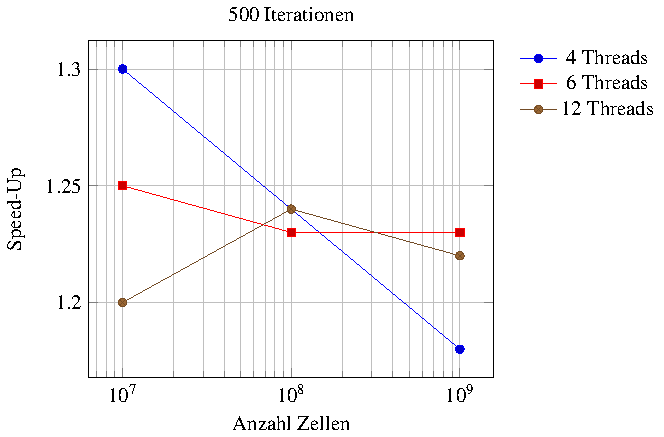
\includegraphics{papers/parallelisierung/images/speedup500.pdf}
		\caption{500 Iterationen}
		\label{parallelisierung:fig:Speedup500}
	\end{figure}
	
	
	% 2. Diagramm: 5000 Iterationen
	\begin{figure}
		\centering
		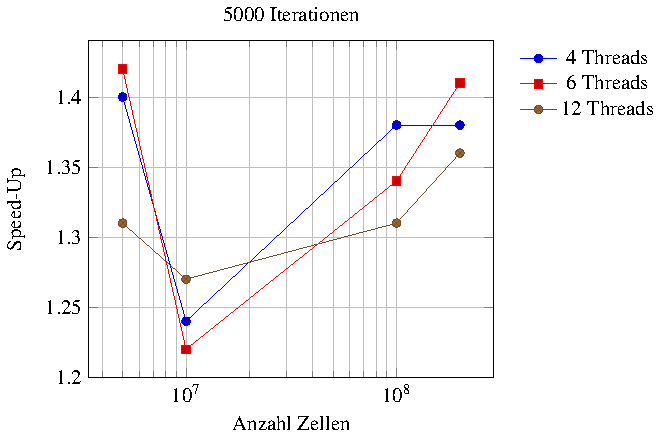
\includegraphics{papers/parallelisierung/images/speedup5000.pdf}
		\caption{5000 Iterationen}
		\label{parallelisierung:fig:Speedup5000}
	\end{figure}
	
	
	% 3. Diagramm: 10000 Iterationen
	\begin{figure}
		\centering
		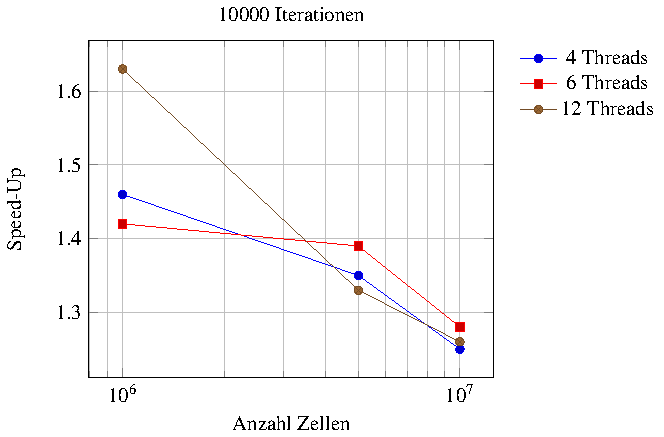
\includegraphics{papers/parallelisierung/images/speedup10000.pdf}
		\caption{10000 Iterationen}
		\label{parallelisierung:fig:Speedup10000}
	\end{figure}
	

Der Speed-Up ist in allen Beispielen ziemlich bescheiden.
Dennoch lassen sich daraus einige Erkenntnisse ziehen.

Bei kleineren Problemen ist der Speed-Up schlechter, wenn mehr Kerne verwendet werden.
Das ist darauf zurückzuführen, dass der Parallelisierungsoverhead mit der Anzahl Kerne unterproportional stark im Vergleich zum Gewinn steigt.
Es ist anzunehmen, dass der Speed-Up mit der Grösse des Problems steigt.
Leider brauchten bereits diese Berechnungen bis zu 30 Minuten pro Rechnung, weshalb noch grössere Rechnungen schwierig durchzuführen waren.

Interessanterweise scheint der Speedup schlechter zu werden, wenn mehr Zellen berechnet werden müssen, jedoch steigt die Effizienz, wenn mehr Iterationen durchgeführt werden.
Eine logische Erklärung hierfür ist, dass das Programm memory bound ist.
Die durchgeführten Operationen sind sehr einfach, wodurch das Auslesen der Daten das Programm ausbremst.
Dadurch kann kein höherer Speedup erreicht werden, da mehr Rechenleistung nichts nützt.

In Abbildung \ref{parallelisierung:fig:Speedup5000} ist ist gut zu erkennen, wie der Speedup bei $10 \cdot 10^6$ im Vergleich zu $5 \cdot 10^6$ sinkt.
Eine naheliegende Erklärung ist, dass ab $10^7$ Einträge die Datenmenge zu gross wird für den Level 3 Cache des Prozessors und damit die Daten im Hauptspeicher abgelegt werden.
Die Zugriffe auf den Hauptspeicher sind bedeutend langsamer, was das memory bound Programm weiter ausbremst.

Für einen besseren Speed-Up müssen die Operationen der einzelnen Iterationen komplex genug sein, damit das Programm durch die Berechnung und nicht durch die Datenzugriffe begrenzt ist.
Die Parallelisierung ist daher für dieses Problem nicht geeignet.
Zur Überprüfung haben wir die Berechnungen künstlich komplexer gemacht.
Diese im Codeabschnitt gezeigte Berechnung hat keinen physikalischen oder mathematischen Hintergrund und dient rein zur Überprüfung dieser These.

\begin{lstlisting}
writeGrid[center] = readGrid[center]*readGrid[center]*readGrid[center]*6.2 +
					lambda * (readGrid[north]*9.11 + readGrid[south]*9.11 +
					readGrid[east]*5.3 + readGrid[west]*3.7 -
					4.0 * readGrid[center]);	
\end{lstlisting}

Mit 4 Threads, $10^6$ Einträgen und $10^5$ Iterationen erhält man 
\bgroup
\small
\begin{verbatim}
================================================
PERFORMANCE VERGLEICH
================================================
Serielle Zeit:   52.5121 Sekunden
Parallele Zeit:  15.6462 Sekunden
------------------------------------------------
SPEEDUP:         3.36x
EFFIZIENZ:       83.9%
------------------------------------------------
\end{verbatim}
\egroup
Man sieht, dass mit dieser Anpassung der Speedup bedeutend besser wird.
Das Programm ist demnach tatsächlich memory bound.
